% uncomment this to use pubform
%\documentstyle[psfig, amsmath]{pubform}

\documentclass[psfig]{sig-alternate}

\begin{document}

\title{StreamIt: A Compiler for Streaming Applications}

% uncomment this to use pubform
%% \author{Bill Thies, Michal Karczmarek, Michael Gordon, David Maze, Jeremy Wong, \\ Henry Hoffmann, Matthew Brown, and Saman Amarasinghe \\
%% \parbox{6in}{\centering{Laboratory For Computer Science\\
%%     Massachusetts Institute of Technology\\
%%     Cambridge, MA  02139\\
%%     \tt{\{thies, karczma, mgordon, dmaze, jnwong, hank, morris, saman\}@lcs.mit.edu}}}}
%% \date{\today}

\numberofauthors{1}
\author{
\alignauthor \vspace{-18pt}
Bill Thies, 
Michal Karczmarek, 
Michael Gordon, 
David Maze, 
Jeremy Wong,
Henry Hoffmann, 
Matthew Brown, 
and Saman Amarasinghe\\
	\vspace{6pt}
	Laboratory for Computer Science \\
	Massachusetts Institute of Technology \\
	Cambridge, MA  02139 \\
%	\vspace{6pt}
%	{\tt \{thies, karczma, mgordon, dmaze, jnwong, hank, morris, saman\}@lcs.mit.edu} \\
%	\vspace{12pt}
%        \today
}

% for the arrow of a function def, etc.
\newcommand{\ma}[2]{max_{#1 \rightarrow #2}}
\newcommand{\mi}[2]{min_{#1 \leftarrow #2}}
\newcommand{\floor}[2]{\left\lfloor\frac{#1}{#2}\right\rfloor}
\newcommand{\ceil}[2]{\left\lceil\frac{#1}{#2}\right\rceil}
\newtheorem{definition}{Definition}
\newtheorem{theorem}{Theorem}

\newcommand{\ra}[0]{\rightarrow}

\maketitle

\begin{abstract}
%Applications that are structured around some notion of a "stream"
are becoming increasingly important and widespread.  There is
evidence that streaming media applications are already consuming
most of the cycles on consumer machines \cite{Rix98}, and their
use is continuing to grow.  {\StreamIt} is a language and compiler
specifically designed for modern stream programming.  Despite the
prevalence of these applications, there is surprisingly little
language and compiler for practical, large-scale stream
programming.  {\StreamIt} is a language and compiler specifically
designed for modern stream programming.  The {\StreamIt} langauge
holds two goals: first, to provide high-level stream abstractions
that improve programmer productivity and program robustness within
the streaming domain; second, to serve as a common machine
language for grid-based processors.  At the same time, {\StreamIt}
compiler aims to perform stream-specific optimizations to achieve
the performance of an expert programmer.  This thesis develops
several techniques for scheduling execution of {\filters} in
{\StreamIt}.  The work focuses on correctness as well as
minimizing buffering requirements and stored schedule size.

\end{abstract}

%\section{Introduction}

The domain of stream programs is important because it stands at the
intersection of trends in applications and architectures.  Stream
programming naturally represents applications such as audio, video,
digital signal processing, and data analysis; applications that are
increasing prevalent as computing moves towards data-centric
applications and to the mobile and embedded space.  Also, by virtue of
their structure -- a graph of independent computational nodes (termed
{\it filters}) with explicit and regular communication -- stream
programs are a natural fit for exploiting coarse-grained parallelism
suitable for multicore architectures.  The interest in streaming
applications has spawned a number of streaming languages that target
the streaming domain, including StreamIt~\cite{streamitcc},
Brook~\cite{brook04}, Cg~\cite{cg03},
SPUR~\cite{spur05samos}, Spidle~\cite{spidle03}, Lime~\cite{lime10},
and SPL~\cite{spl09}.

In a stream program, filters define an atomic execution step that
repeats for many iterations; each execution step discards a number of
data items from filter's input edge.  Often, a filter does not discard
all the data items that it read for the current execution step,
requiring these inspected (but not discarded) items for a future
iteration (or iterations) of the filter.  This type of filter is
described as performing a sliding window computation on its
input. Sliding window computations are prevalent in stream programs.
Examples of sliding window computations include FIR filters; moving
averages and differences; error correcting codes; motion estimation;
and network packet inspection.  A recent study of a large streaming
benchmark suite written in the StreamIt programming language finds
that 17 of the 30 real-world benchmarks include at least one filter
that performs a sliding window computation~\cite{streamit-suite}.


Figure~\ref{fig:fir-nopeeking} shows how to perform a sliding
window FIR filter via state carried between iterations of a filter.
This implementation is difficult for the compiler to analyze and
reason about.  Some programming languages (e.g., Brook, Lime,
StreamIt, and IBM SPL) go so far as to include idioms that directly
represent sliding window computation, allowing the programmer to
specify, for each filter, the size of the window and the number of
items discarded after an execution of the filter.
Figure~\ref{fig:fir-peeking} shows how language extensions of the
StreamIt programming language elegantly expose sliding windows for
compiler analysis and optimization.

A goal of stream programming is to directly expose to the software
layer the necessary information to enable automatic management of
coarse-grained parallelism.  Stream programs expose multiple forms of
parallelism: pipeline parallelism that exists between producers and
consumers; task parallelism that exists between pairs of filters on
parallel branches of the stream graph; and data parallelism that
exists when a filter is stateless and can thus be replicated.  Data
parallelism is the most attractive, as it provides load-balanced and
limitless parallelism (as long as input data is available).  A filter
that is stateful, and cannot be data-parallelized, becomes a limit to
parallelization scalability, as the work of that filter cannot be
divided; the most load-intensive stateful filter becomes a
bottleneck.

This paper presents a compiler framework for data-parallelizing
filters that perform sliding window computations when the properties
of the sliding window can be calculated statically.  If sliding window
filters required state, this state would represent a new
parallelization bottleneck.  Sliding windows are the bottleneck in 11
of the 17 real-world benchmarks in the StreamIt Benchmark Suite that
contain sliding windows~\cite{streamit-suite}.  For example, examining
the Channelvocoder benchmark, this state would limit scalability to 18
cores, whereas our techniques scale to at least 64 cores.

Data-parallelizing a filter is performed via a transformation termed
{\it fission} (verb form {\it fiss})~\cite{streamit-asplos}.  Fission
is the process of data-parallelizing a stateless filter by duplicating
the filter a certain number of ways, assigning duplicates to distinct
cores, and correctly distributed input data to and collecting output
data from the duplicates.  The duplicated filters are referred to as
{\it products}.  When a sliding window is present, fission is
accomplished by duplicating certain input items since they are
required by multiple products.  This duplication translates into
inter-core communication, a limiting factor for scalability when
targeting multicore architectures.

Previous approaches duplicate each input data item to all products,
with products ignoring (decimating) items that are not
needed~\cite{streamit-asplos}.  We will show that this strategy limits
scalability for multicores by requiring too much inter-core
communication.  In contrast, our strategy precisely routes each input
item to the minimal set of product filters that requires the item.
Unlike previous work, our techniques are defined on
multiple input and multiple output filters, removing the need to
introduce synchronization filters that serialize data before and
after the product filters.  

Our techniques operate on {\it static-rate} stream graphs, meaning
that the number of items produced, the number of items consumed, and
the number of items inspected by each filter can be determined
statically.  Because of this property, a steady-state schedule of
filter firings can be calculated that does not grow buffers and can be
executed indefinitely~\cite{lee87}.  Our techniques are conscious of
the spatial locality between producers and consumers.  Our framework
includes techniques that can determine when spatial locality can be
increased by altering the steady-state schedule.  When applicable, our
techniques can reduce the overall sharing (and thus inter-core
communication) requirement to below a threshold percent of the total
input communication for each sliding window filter that is
data-parallelized. 

\begin{figure}[t]
\centering
\subfigure[]{\includegraphics[width=3.3in]{figures/fir-nopeeking.pdf}\label{fig:fir-nopeeking}}
\subfigure[]{\includegraphics[width=3.3in]{figures/fir-peeking.pdf}\label{fig:fir-peeking}}
\caption[Two implementations of an FIR filter.]{\label{fig:fir-code}
  Two StreamIt implementations of an FIR filter:
   (a) the non-peeking version implemented via a
  stateful circular buffer; and (b) the peeking version. Only steady-state implementation is
  given.}
\end{figure}

The framework presented is defined on a model of computation that is
agnostic of source language.  To evaluate our techniques we have
implemented them in the context of the StreamIt compiler
infrastructure~\cite{gordon-asplos06}.  Our transformations are guided
by the parallelization management techniques presented
in~\cite{gordon-asplos06}.  We employ 3 real-world benchmarks from the
StreamIt Benchmark Suite~\cite{streamit-suite} that include sliding
window computation.  We demonstrate the effectiveness of our
techniques by comparing them to previously published techniques on 2
multicore architectures: a 16-core SMP shared-memory multicore and the
64-core distributed-memory Tilera TILE64.  We show that
our techniques are required to achieve scalable parallelization on
both architectures, achieving a 6.7x mean speedup on the 16-core SMP
and a 1.8x mean speedup on the 64-core distributed memory multicore
over a previously published technique.

\subsection{Contributions}
This paper makes the following contributions:
\begin{itemize}
  % \myitem{Motivation for Exposing Sliding Windows in Stream
  %   Languages}: Without exposing sliding windows in the language, it
  % requires heroic effort by the compiler to analyze the access patterns
  % of such a filter. Without success, the compiler will not be able to
  % data-parallelize these filters.  This will prevent robust 
  % parallelization scalability for streaming applications.

  \myitem{Generalized Fission of Sliding Window Filters}: We present a
  transformation that fisses sliding window filters with multiple
  input and multiple outputs.  The technique also supports filters
  that with multiple schedules of execution.  General fission defines
  a precise pattern of communication of input data to the products
  that can be reasoned upon by our other techniques.

  \myitem{Sharing Reduction}: We are the first to present a technique
  that decides when it is possible to decrease the amount of sharing
  between fission products by altering the steady-state of a stream
  graph, thus decreasing inter-core communication.  The technique
  reasons about all the sliding window filters of the stream graph,
  and when possible, reduces the sharing requirement to below a given
  threshold percent of the total input of the filters. 

  \myitem{Data Parallelization of Stream Graph}: We present a
  framework for data-parallelizing all of the filters of a stream
  graph employing the fission transformation on individual filters and
  applying sharing reduction when possible.  This framework optimizes
  for spatial locality and enables the compiler to automatically and
  effectively manage parallelization across varying multicore
  architectures.

  \myitem{Enable Robust Parallelization Scaling for Multicores}: For
  streaming applications with sliding window computation, previously
  published data-parallelization transformations do not scale for our
  target multicores. Our techniques enable robust parallelization
  scalability by reducing inter-core communication.  We achieve a 17x
  mean parallelization speedup for a 16-core SMP and a 62.3x mean
  parallelization speedup for the 64-core TILE64 across our benchmarks.

\end{itemize}

% \begin{figure}[t]
% \centering
% \begin{subfloat}
% \begin{minipage}[b]{0.45\textwidth}
% \eightpoint
% \begin{verbatim}
% float->float filter FIR(int N) {
%   int srcBuffer[N];
%   int srcEnd = 0; 
%   ...
%   work push 1 pop 1 {
%     srcBuffer[srcEnd] = pop();
%     float sum = 0;
%     for (int i=0; i<N; i++) {
%       sum += weights[i] * srcBuffer[(srcEnd + i + 1) % N];
%     }
%     push(sum);
%     srcEnd = (srcEnd + 1) % N;
%   }
% }
% \end{verbatim}
% \vspace{-8pt}
% \end{minipage}%
% \caption{ \label{fig:fir-nopeeking}}
% \end{subfloat}%
% \qquad
% \begin{subfloat}
% \begin{minipage}[b]{0.45\textwidth}
% \eightpoint
% \begin{verbatim}
% float->float filter FIR(int N) {
%   ...
%   work push 1 pop 1 peek N {
%     float sum = 0;
%     for (int i=0; i<N; i++) {
%       sum += weights[i] * peek(i);
%     }
%     push(sum);
%     pop();
%   }
% }
% \end{verbatim}
% \vspace{-18pt}
% \end{minipage}
% \caption{ \label{fig:fir-streamit}}
% \end{subfloat}
% \caption[Two implementations of an FIR filter.]{\label{fig:fir-code}
%   Two StreamIt implementations of an FIR filter:
%    \subref{fig:fir-nopeeking} the non-peeking version implemented via a
%   stateful circular buffer; and \subref{fig:fir-streamit} the peeking version. Only steady-state implementation is
%   given.}
% \end{figure}

%\Section{StreamIt Programming Language}
\label{sec:streamit}

StreamIt~\cite{streamit-cc} is an architecture independent language
that is designed for stream programming. In StreamIt, programs are
represented as graphs where nodes represent computation and edges
represent FIFO-ordered communication of data over tapes. The language
features several novelties that are essential for large scale program
development. The language is modular, parameterizable, malleable and
architecture independent. In addition, the language exposes the
inherent parallelism and communication patterns that are prevalent in
streaming programs.

\begin{figure*}[t]
  \begin{minipage}[t]{4.0in}
    {
	\begin{scriptsize}
	  \begin{verbatim}
	    int->int filter ZigZagScan(int N, int[N] Order)
	    {
	        work pop N push N {
	        for (int i = 0; i < N; i++) {
	          int pixel = peek(Order[i]);
	          push(pixel);
	        }
	        for (int i = 0; i < N; i++) {
	          pop();
	        }
	      }
	    }
	  \end{verbatim}
	\end{scriptsize}
    }
    % \vspace{-3pt}
    \caption{Example filter implementing zig-zag scanning.}
    % \label{fig:zigzag-filter}
  \end{minipage}
  ~~\vrule~~
  \begin{minipage}[t]{3.0in}
    {  
	\begin{scriptsize}
	  \begin{verbatim}
	    int[64] Ordering = 
	      {00, 01, 05, 06, 14, 15, 27, 28,
	       02, 04, 07, 13, 16, 26, 29, 42,
	       03, 08, 12, 17, 25, 30, 41, 43,
	       09, 11, 18, 24, 31, 40, 44, 53,
	       10, 19, 23, 32, 39, 45, 52, 54,
	       20, 22, 33, 38, 46, 51, 55, 60,
	       21, 34, 37, 47, 50, 56, 59, 61,
	       35, 36, 48, 49, 57, 58, 62, 63};



	  \end{verbatim}
	\end{scriptsize}
    }
    % \vspace{-3pt}
    \caption{Example zig-zag order for filter.}
    \label{fig:zigzag-order}
  \end{minipage}
\end{figure*}

\SubSection{Filters as Programmable Units}
In StreamIt, the basic programmable unit is a {\it filter}. Each
filter contains a work function that executes atomically, popping
(i.e., reading) a fixed number of items from the filter input tape
and pushing (i.e., writing) a fixed number of items to the filter
output tape. A filter may also {\tt peek} at a given index on its
input tape without consuming the item; this makes it simple to
represent computation over a sliding window or performing permutations
on the input stream. The {\tt push}, {\tt pop}, and {\tt peek} rates
are declared as part of the work function, thereby enabling the
compiler to apply various optimizations and construct efficient
execution schedules. 

A filter is akin to a class in object oriented programming with the
work function serving as the main method. A filter is parameterizable,
and this allows for greater malleability and code reuse. An example
filter is shown in Figure~\ref{fig:zigzag-filter}. This filter
consumes a stream whose elements are of type {\tt int} and produces a
stream of the same type. It implements the zig-zag scanning pattern
used in the run-length encoding of quantized DCT coefficients (see
Figure~\ref{fig:zigzag}). Typically, the zig-zag scan operates on a
8x8 matrix. An instantiation of a filter can specify the matrix
dimensions, as well as the desired ordering. In MPEG, there are two
possible scan orders. The {\tt Order} parameter can define the
specific scan pattern that is desired. For example, to implement the
order shown in Figure~\ref{fig:zigzag}(a), the array is defined as
shown in Figure~\ref{fig:zigzag-order}.

In this example, the DCT matrix is represented as a unidimensional
stream. The filter peeks or inspects the elements and copies them to
the output stream in the specified order. Once all the DCT
coefficients are copies, the input stream is deallocated from the tape
with a series of pops.

\begin{figure}[t]
\begin{center}
%\vspace{-24pt}
% \framebox{
 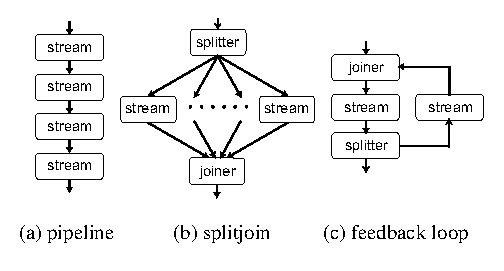
\includegraphics[scale=1, angle=0]{./constructs-eg.eps}
%}
% \vspace{-6pt}
% \nocaptionrule
 \caption{Hierarchical streams in StreamIt.}
 \label{fig:containers}
\end{center}
\end{figure}

\SubSection{Hierarchical Streams}
In StreamIt, the application developer focuses on the hierarchical
assembly of the stream graph and its communication topology, rather
than on the  explicit management of the data buffers between filters.
StreamIt provides three hierarchical structures for composing filters
into larger stream graphs (see Figure~\ref{fig:containers}).

\paragraph{Pipeline.}
The {\it pipeline} stream construct composes streams in sequence, with
the output of one connected to the input of the next.  An example of a
pipeline appears in Figure~\ref{fig:decoder-pipeline}. A pipeline is a
single input to single output stream. The decoding pipeline in the
figure consists of three streams. The first is a filter which zig-zag
unorders the input stream, and prepares the data for the inverse
quantization and DCT. The output of the filter is consumed by a stream
named {\tt IQ} which is a pipeline itself (not shown). This example
illustrates the hierarchical nature of stream composition in
StreamIt. The {\tt IQ} pipeline performs the inverse quantization, and
produces an output stream that is in turn consumed by another stream
which performs the inverse DCT. As in the case of a filter, pipelines
are also parameterizable.

\begin{figure*}[t]
  \begin{scriptsize}
    \begin{verbatim}
	int->int pipeline Decode()
	{ 
	  int Order[64] = {...};     // initialized as shown earlier
	  add ZigZagScan(64, Order);
	  add IQ();                  // inverse quantization
	  add IDCT(8, 8);            // inverse DCT (8x8 matrix)
	}
    \end{verbatim}
  \end{scriptsize}
  % \vspace{-3pt}
  \caption{Example MPEG decoder pipeline.}
  \label{fig:decoder-pipeline}
\end{figure*}

The {\tt add} keyword in StreamIt constructs the specified stream
using the input parameters. The {\tt add} statement may only appear in
non-filter streams.  In essence, filters are the leaves in the
hierarchical construction, and composite nodes in the stream graph
define the encapsulating containers. This allows for modular design
and development of large applications, thereby  promoting
collaboration, increasing code reuse, and simplifying debugging.

\paragraph{Split-Join.}
The {\it splitjoin} stream construct distributes data to a set of
parallel streams, which are then joined together in a roundrobin
fashion. In a splitjoin, the {\it splitter} performs the data
scattering, and the {\it joiner} performs the gathering. A splitter is
a specialized filter with a single input and multiple output
channels. On  every execution step, it can distribute its output to
any one of its children in either a {\it duplicate} or a {\it
roundrobin} manner. For the former, incoming data are replicated to
every sibling connected to the splitter. For the latter, data are
scattered in a roundrobin manner, with each item sent to exactly one
child stream, in order. The splitter type and the weights for
distributing data to child streams are declared as part of the syntax
(e.g., \texttt{split duplicate} or \texttt{split
roundrobin($w_1,\ldots,w_n$)}). The splitter counterpart is the
joiner. It is a specialized filter with  multiple input channels but
only one output channel. The joiner gathers data from its predecessors
in a roundrobin manner (declared as part of the syntax) to produce a
single output stream.

\begin{figure*}[t]
  \begin{scriptsize}
    \begin{verbatim}
	// N = macroblock size + motion vector data size;
	// W = picture width (resolution in pixels);
	// H = picture width (resolution in pixels);

	int->int splitjoin YCrCbDecoding(int N, int W, int H)
	{
	  // 4:2:0 chroma format
	  split roundrobin(4*N, 1*N, 1*N);

	  add LuminanceChannel  (W, H);
	  add ChrominanceChannel(W, H);
	  add ChrominanceChannel(W, H);

	  join roundrobin(1, 1, 1);  
	}
    \end{verbatim}
  \end{scriptsize}
  % \vspace{-3pt}
  \caption{Example MPEG decoder splitjoin.}
  \label{fig:decoder-sj}
\end{figure*}

The splitjoin stream is a convenient and natural way to represent
parallel computation. For example, when the decoder performs the
luminance and chrominance channel processing, the computation can
occur in parallel. In StreamIt, this is expressed as shown in
Figure~\ref{fig:decoder-sj}. The input stream contains the
macroblock data along with the parsed motion vectors. The data is
partitioned and passed to one of three decoding channels, with $4N$
items assigned to the first stream, $N$ items to the second, and $N$
items to the third. The three streams reconstruct the original
pictures with respect to the different color channels, and their
output is combined by the joiner to produce the final decoded picture.

\paragraph{Feedback Loop.}
StreamIt also provides a {\it feedback loop} construct for introducing
cycles in the graph. This stream construct is not used in the decoder,
but may be used in the MPEG encoder.

\paragraph{XXX: need to introduce messaging and talk about it.}
\begin{figure}
\centering
\psfig{figure=tapes.eps,width=3.2in}
\caption{A filter's input and output tapes during an execution step.
With each step, the filter pushes two items, pops two items, and peeks
at three additional items.  The initial state of the input tape is
shown at left.  The center shows the filter with both input and output
tapes during the invocation of {\tt work}.  The final state of the
output tape is shown at right.}
\label{fig:tape}
\end{figure}

\begin{figure}
\centering
\psfig{figure=pipeline.eps,width=2.0in}

(a) A Stream. \\
\vspace{8pt}
\psfig{figure=splitjoin.eps,width=3.2in}

(b) A SplitJoin. \\
\vspace{8pt}
\psfig{figure=feedback.eps,width=3.2in}

(c) A FeedbackLoop. \\
\vspace{8pt}
\caption{Tape labeling for StreamIt structures.}
\label{fig:tapelabels}
\end{figure}

\section{Streaming Model of Computation}

In this section, we develop an abstract model of streaming computation
to serve as a basis for reasoning about program transformations and
compilation techniques within the streaming domain.  A stream graph
differs from a traditional, sequential program in that all of the
filters of the graph are implicitly running in parallel, with the
execution order constrained only by the availability of data on
channels between the filters.  Further, filters communicate only with
their immediate neighbors, thereby removing any notion of global time
or non-local dependences of one filter on another.  [add idea that it
is the specification of the atomic work function that really prevents
global time] These properties merit the development of a new model of
computation, in which the notions of timing, scheduling, and
dependence analysis are in terms that are relative to a given filter
in the graph, instead of being global characteristics of a program.

In Section \ref{minfunc}, we develop a transfer function that provides
the basis for distributed time in a stream graph... [build operational
semantics to give a precise meaning to messaging, and denotational
semantics to validate program transformations].

\subsection{Notation}

We use the following notation:

\begin{itemize}

\item A {\it tape} is an infinite history of the values that have been
  pushed onto a channel between two filters (see Figure
  \ref{fig:tapes}).  We use $I_A$ and $O_A$ to denote the input and
  output tapes of filter $A$, respectively, with numbering used to
  distinguish between multiple input or output tapes (see Figure
  \ref{tapelabels}).  Finally, $n(T)$ represents the number of items
  on tape $T$ at a given point of execution.  [should we define $p(T)$
  here or wait until we use it?  long time def-use!]

\item We say that filter $A$ is {\it upstream} of filter $B$ (or,
  equivalently, $B$ is {\it downstream} $A$) if there is a directed
  path in the stream graph from $O_A$ to $I_B$.

\item The number of items that are pushed, popped, and peeked by
  filter $A$ during a single execution of its work function are
  denoted by $push_A$, $pop_A$, and $peek_A$, respectively.  Note that
  $peek_A$ includes the items that are popped, such that $pop_A \le
  peek_A$.

\end{itemize}

\subsection{Relative Time}
\label{sec:minfunc}

As outlined above, there is no concept of global time in a stream
graph since each filter is completely independent and can only
communicate with its neighbors through input and output channels.
Thus, if two filters need to synchronize an event, the synchronization
must be in terms of the data items that are passed over a channel.

In this context, we define a $min$ function between tapes in the
stream graph that allows disconnected filters to have a common notion
of time.  The function is defined in terms of data dependence:
\begin{definition}
$\mi{a}{b}(x)$ is the minimum number of items that must appear on tape
$a$ given that there are $x$ items on tape $b$.
\end{definition}

We now turn to deriving $\mi{a}{b}$ for all pairs of tapes $a$ and $b$
in a filter graph where $a$ is upstream of $b$.

\subsubsection{Filters}

Let us derive $\mi{I_A}{O_A}(x)$, which represents the time shift
across a single filter $A$.  Since the filter produces $push_A$ items
on every invocation, it must be invoked
$\left\lceil\frac{x}{push_A}\right\rceil$ to produce the $x$'th item.
On each invocation, it consumes $pop_A$ items, and peeks at an
additional $peek_A-pop_A$ items.  Thus, the total number of items that
must be present on the input is:
\begin{align*}
\mi{I_A}{O_A}(x) = \left\lceil\frac{x}{push_A}\right\rceil*pop_A+(peek_A-pop_A)
\end{align*}

\subsubsection{Pipelines}

Let us now derive an expression for $min$ in the case of a pipeline.
In the base case, consider that two filters are connected, with the
output of $A$ feeding into the input of $B$ (see
Figure~\ref{fig:tapelabels}).  We are seeking $\mi{I_A}{O_B}(x)$: the
minimum number of items that must appear on tape $I_A$ given that
there are $x$ items on tape $O_B$.  Observing that a minimum of
$\mi{I_B}{O_B}(x)$ items must appear on tape $I_B$, and that $I_B$
must equal $O_A$ since the filters are connected, we see that a
minimum of $\mi{I_A}{O_A}(\ma{I_B}{O_B}(x))$ items must appear on
$I_A$:
\begin{align*}
\ma{I_A}{O_B} = \mi{I_A}{O_A} \circ \mi{I_B}{O_B}
\end{align*}
By identical reasoning, this composition law holds for pipelined
streams as well as filters.  That is, given tapes $x$, $y$, and $z$,
we have that:
\begin{align}
\label{eq:compose}
\mi{x}{z} &= \mi{x}{y} \circ \mi{y}{z}
\end{align}
However, there is a restriction on this definition.  It only applies
when there is a downstream path $P_1$ from the filter following $x$ to
the filter preceding $y$, a downstream path $P_2$ from the filter
following $y$ to the filter preceding $z$, and the paths $P_1$ and
$P_2$ are non-overlapping.  This restriction prevents the successive
composition of transfer functions around feedback loops, thereby
ensuring a unique definition for all pairs $(x, z)$ where there is a
downstream path from $x$ to $z$.

\subsubsection{SplitJoins}

\subsubsection{FeedbackLoops}

%% \subsubsection{SplitJoins}

%% We now derive $min$ and $max$ in the case of a SplitJoin, as pictured
%% in Figure \ref{splitjoin}.  For the splitter $S$ there are two output
%% tapes; let us denote them by $O1_S$ and $O2_S$.  Similarly, let us
%% denote the two input tapes of the joiner $J$ by $I1_J$ and $I2_J$.  We
%% derive below the transfer functions the round robin and
%% duplicate/combine nodes.  Note that the duplicate/combine nodes can be
%% simulated with round robins and duplicating filters, but we provide
%% the transfer functions anyways to simplify the semantic analysis of a
%% program.  We have yet to derive these expressions for the weighted
%% round robin nodes.

%% {\bf Round robin splitter.}  In the case of a round-robin splitter, the
%% items from the input tape are alternately routed to the output tapes,
%% with the first item going onto tape $O1_S$.  By this definition, we
%% can see that the splitter's $max$ is defined as follows:
%% \begin{align*}
%% \ma{I_S}{O1_S}(x) &= \left\lceil\frac{x}{2}\right\rceil \\
%% \ma{I_S}{O2_S}(x) &= \left\lfloor\frac{x}{2}\right\rfloor
%% \end{align*}
%% To derive the $min$ function across a splitter, observe that the input
%% tape need only progress so far as to produce the items on the emptier
%% output tape.  That is, we need to consider the number of items on both
%% of the splitter's output to determine the minimum number of items that
%% are needed at its input.  Thus, our $min$ function has two arguments:
%% the first corresponding to $O1_S$ and the second corresponding to
%% $O2_S$.  The equation is as follows:
%% \begin{align*}
%% \mi{I_S}{(O1_S, O2_S)}(x_1, x_2) = MIN(2*x_1-1, 2*x_2)
%% \end{align*}
%% {\bf Round robin joiner.}  The rules for a round robin joiner are in
%% some sense dual to those of the round robin splitter.  Again assuming
%% that items are alternately drawn from the input tapes, starting with
%% $I1_J$, we have that:
%% \begin{align*}
%% \mi{I1_J}{O_J}(x) &= \left\lceil\frac{x}{2}\right\rceil \\
%% \mi{I2_J}{O_J}(x) &= \left\lfloor\frac{x}{2}\right\rfloor
%% \end{align*}
%% Again, the $max$ function takes two arguments, corresponding to the
%% number of items on $I1_J$ and $I2_J$, respectively:
%% \begin{align*}
%% \ma{(I1_J, I2_J)}{O_J}(x_1, x_2) = MIN(2*x_1-1, 2*x_2)
%% \end{align*}
%% {\bf Duplicate splitter}.  Clearly, the $max$ function of a duplicate
%% splitter is simply the identity function, since it maps each element
%% on the input tape to the same location on the output tapes:
%% \begin{align*}
%% \ma{I_S}{O1_S}(x) &= x \\
%% \ma{I_S}{O2_S}(x) &= x
%% \end{align*}
%% The $min$ function is similar, except that--like the round robin
%% split--the input need only progress as far as the lesser output:
%% \begin{align*}
%% \mi{I_S}{(O1_S, O2_S)}(x_1, x_2) = MIN(x_1, x_2)
%% \end{align*}
%% {\bf Combine joiner.} The combine joiner is simply the dual of the
%% duplicate splitter, with transfer functions that the reader can verify
%% as follows:
%% \begin{align*}
%% \ma{(I1_J, I2_J)}{O_J}(x_1, x_2) &= MIN(x_1, x_2) \\
%% \mi{I1_J}{O_J}(x) &= x \\
%% \mi{I2_J}{O_J}(x) &= x
%% \end{align*}

%% \subsubsection{FeedbackLoops}

%% \begin{figure}
%% \centering
%% \psfig{figure=feedback.eps,width=3.2in}
%% \caption{\protect\small  FeedbackLoop construct with labeling.
%% \protect\label{looplabel}}
%% \end{figure}

%% We have to be careful when defining the transfer functions for
%% feedback loops (see Figure \ref{looplabel}).  The feedback splitter
%% $FS$ serves as a normal splitter, and has the same $min$ and $max$
%% functions as defined above.  However, the feedback joiner $FJ$ is
%% slightly different than a standard joiner, since during the first few
%% executions it fabricates values from the loop body before they appear
%% on the input tape.  The transfer function must take special account of
%% these initial values, since they never appear on $I2_{FJ}$, the input
%% tape from the loop body.  This is because we model the initialization
%% of FeedbackLoops by feeding the joiner the initial values directly
%% instead of pushing them onto a channel.

%% Let $n$ be the number of initial values that are provided to the
%% feedback joiner before values from the feedback loop are read.  Let
%% $J$ be a normal COMBINE or ROUND\_ROBIN joiner as defined for
%% SplitJoins.  Now, let us define the transfer functions for $FJ$, the
%% feedback joiner.

%% The $min$ function for the main stream is as before:
%% \begin{align*}
%% \mi{I1_{FJ}}{O_{FJ}} = \mi{I1_J}{O_J} 
%% \end{align*}
%% However, we must offset by $n$ when considering the $min$ function
%% that draws from the loop's tape:
%% \begin{align*}
%% \mi{I2_{FJ}}{O_{FJ}}(x) = \mi{I2_J}{O_J}(x) - n
%% \end{align*}
%% Finally, the $max$ function must be similarly shifted for the input
%% from the loop:
%% \begin{align*}
%% \ma{(I1_{FJ}, I2_{FJ})}{O_{FJ}}(x_1, x_2) = \ma{(I1_J, I2_J)}{O_J}(x_1,
%% x_2 + n)
%% \end{align*}

\subsubsection{Program Verification}

Borrow from program verification section of last paper. 

\subsection{Message Timing}

in the previous description of streamit, the messaging system was left
unspecified.  here we use the min function to give a precise semantics
to message delivery timing in streamit.  this will yield an
operational semantics to the scheduling of streamit programs.

\subsection{Operational Semantics}

\subsection{Denotational Semantics}

assume for now that the filters are stateless.

the above discussion addresses the order in which filters can be
executed, but does not address the values on the tapes, or the meaning
of a program as a whole.  for this we turn to a denotational
semantics, which will allow us to prove the equivalence of two
different stream programs.

in the denotaional semantics, we'll represent a filter as follows:

1. push, pop, (max items peeked)
2. the functions specifying the output values as a function of the
input values.

3. this set of functions...

ii. how to map a given textual representation into a canonical
representation.

iii. how to represent the canonical representation in the functinal
format

iv. further, to help automate program transformations, we can talk
about translationg from the functional format to the canonical
representation.  talk about CSE from reconstruction

in the next sections, we'll appeal to this denotational semantics in
argueing for the correctness of program transformations.

\section{Optimization}

then discuss a few optimizations with the denotational semantics to
prove that they are correct


\section{Scheduling}

\begin{figure}
\centering
\psfig{figure=sched_diag.eps,width=3.4in}
\caption{Three different scheduling schemes.}
\label{fig:sched}

\end{figure}

Scheduling the order of the execution of filters has a large impact on 
the behavior of a StreamIt program.  In this section we introduce three
different scheduling techniques and analyze their properties.  The analysis
presented here is quite superficial, as detailed analysis falls outside of
the scope of this paper.

\subsection{Periodic Schedule}
A schedule for a StreamIt program needs to satisfy a requirement that
a repeated execution of the schedule cannot lead to changed data buffering
between filters.  This is a separate constraint from that in section
\ref{sec:prog-verif}:  while it is impossible to produce a valid schedule
for an invalid program, it is quite easy to produce an invalid schedule for
a valid program.  We call a schedule that satisfies these requirement a
periodic schedule.  (Here a schedule represents the multiplicity of executions
of filters, ignoring the ordering of these executions.)

\begin{theorem}
\label{theo:period-sched}
For every valid program, there exists a unique, minimal periodic schedule.
Every other periodic schedule for a StreamIt program is a multiple of the
underlying periodic schedule [\ref{bhat1994x3}].  (the multiple principle
is never clearly stated (I don't think) but I don't want to have to prove
it and I need it)
\end{theorem}

While computing periodic schedules for StreamIt, we chose to preserve the
hierarchical structure presented in the program.

A filter has a periodic schedule of a single execution.  This is because
there are no scheduler-visible buffers inside of a filter.  All other
components of the program express their periodic schedules in terms of
number of executions of their subcomponents necessary to construct a valid
schedule.  This technique relies on Theorem \ref{theo:period-sched} to
assure that the periodic schedule built is indeed the minimal periodic
schedule.

\subsection{Initialization Schedule}

Before we can execute any periodic schedule on a program, the program may
require intialization.  This is because we allow filters with $peek_A$ values
greater than their $pop_A$ values.  If the program is not initialized, a filter
that peeks more than it pops would not be able to consume all the input 
provided for it during the first execution of a periodic schedule.  The
subsequent executions would force the filter to consume the exact same amount
of data, eventually causing buffer overflow.

The initialization schedule is computed by ensuring that every filter $A$ has
at least $peek_A - pop_A$ unread data on its input tape available after 
initialization has been completed.

\subsection{Single Appearance Schedule}

A single appearance schedule is a schedule in which every filter and every
structure appears exactly once.  Groups of filters and structures can be
combined together to form bigger structures.  In our approach, we chose to
perserve the structuring of the original program when selecting structures
to be grouped together.  Thus a schedule for a given structure is a list
of tuples of components included in this structure and corresponding number
of times each of these components needs to be executed in a given periodic
schedule. (Better results for buffer size have been presented in 
\ref{somepaper}, they are however within the same order of magnitude.)

As an example, the pipeline in Figure \ref{fig:sched} has a schedule
$(4A)(6B)(9C)(3D)$.

\subsection{Minimum Latency Scheduling}




%\mysection{Related Work}
\label{sec:related}

This paper builds directly on the work done to analyze and optimize
linear components in StreamIt graphs \cite{Lamb}. We extend the
theoretical framework for linear analysis to state space analysis in
order to apply our optimizations to a wider class of applications.
Specifically, state space analysis applies to filters with persistent
state, and feedback loops can be combined into a single state space
representation; neither of these cases are handled by linear analysis.
The extension from linear analysis to state space analysis required a
fundamental change to the underlying representation, as well as a
complete reformulation of the rules for combination and expansion.
Moreover, this paper introduces novel optimizations of state removal
and minimal parameterization, both of which operate on the state space
representation.

Several other groups are researching methods for automated DSP
optimizations. SPIRAL \cite{Spiral} is a system developed to generate
libraries of DSP transforms. These libraries are designed for specific
architectures, and can be re-optimized when hardware is upgraded or
replaced. Other such libraries that have been designed include a
package for linear algebra manipulations by the ATLAS project
\cite{Atlas} and portable high-performance FFTs (Fast Fourier
Transforms) \cite{fftw}.

Aside from StreamIt, other programming languages have been designed
for streaming data. Synchronous languages which target embedded
applications include LUSTRE \cite{Lustre}, Esterel \cite{Esterel}, and
Signal \cite{Signal}. Other stream-based languages are Occam
\cite{Occam}, SISAL \cite{sisal}, and StreamC \cite{streamc}.  Some of
these languages are designed to exploit vector and parallel
processing. However, none of these languages have compilers that run
state space or linear analysis.

%\section{Conclusion}

This paper shows that the inter-node dependences of a Cyclo-Static
Dataflow Graph can be cleanly represented as a System of Affine
Recurrence Equations.  In combination with Feautrier's array dataflow
analysis~\cite{Feautrier01} for deducing intra-node dependences, this
establishes the SARE as a unified analysis and optimization framework
for high-level DSP programming models.

We believe that the precise affine dependence framework provided by
the SARE representation will enable a powerful suite of node
optimizations in dataflow graphs.  The SARE is a robust and
well-established framework within the systolic and scientific
communities, with methods for graph parameterization, automatic
parallelization, and storage optimization.  We propose optimizations
such as decimation propagation and node fission that are first
applications of these techniques to the signal processing domain.

%\bibliographystyle{abbrv}
%\bibliography{references}
\end{document}
